\section{Preliminaries}
\label{sec:preliminaries}

This section defines the mathematical concepts used in the paper. Our notation closely follows~\cite{DBLP:conf/edbt/HolschG16} and is similar to~\cite{DBLP:books/igi/Sakr11/RodriguezN11}\footnote{The formalism presented in~\cite{DBLP:books/igi/Sakr11/RodriguezN11} lacks the notion of \emph{vertex labels}.}.

\subsection{Property Graph Data Model}

A \emph{property graph} is defined as $G = (V, E, \verticestoedges, \vertexlabels, \edgelabels, \vertexlabelfunction, \edgelabelfunction, \vertexproperties, \edgeproperties)$, where $V$ is a set of vertices, $E$ is a set of directed edges, $\verticestoedges: E \assign V \cartesianproductop V$ assigns the source and target vertices to edges. The graph is labelled (or typed):
\begin{itemize}
	\item $\vertexlabels$ is a set of vertex labels, $\vertexlabelfunction: V \assign 2^{\vertexlabels}$ assigns \emph{a set of labels} to each vertex.
	\item $\edgelabels$ is a set of edge labels, $\edgelabelfunction: E \assign \edgelabels$ assigns \emph{a single label} to each edge.
\end{itemize}

Furthermore, graph $G$ has properties (\emph{attributed graph}). Let $D$ be a set of atomic domains.
\begin{itemize}
	\item $\vertexproperties$ is a set of vertex properties. A vertex property $p_i \in \vertexproperties$ is a function $p_i: V \assign D_i \unionop \{ \relnull \}$, which assigns a property value from a domain $D_i \in D$ to a vertex $v \in V$, if $v$ has property $p_i$, otherwise $p_i(v)$ returns $\relnull$.
	\item $\edgeproperties$ is a set of edge properties. An edge property $p_j \in \edgeproperties$ is a function $p_j: E \assign D_j \unionop \{ \relnull \}$, which assigns a property value from a domain $D_j \in D$ to an edge $e \in E$, if $e$ has property $p_j$, otherwise $p_j(e)$ returns $\relnull$.
\end{itemize}

\begin{figure}
	\centering
	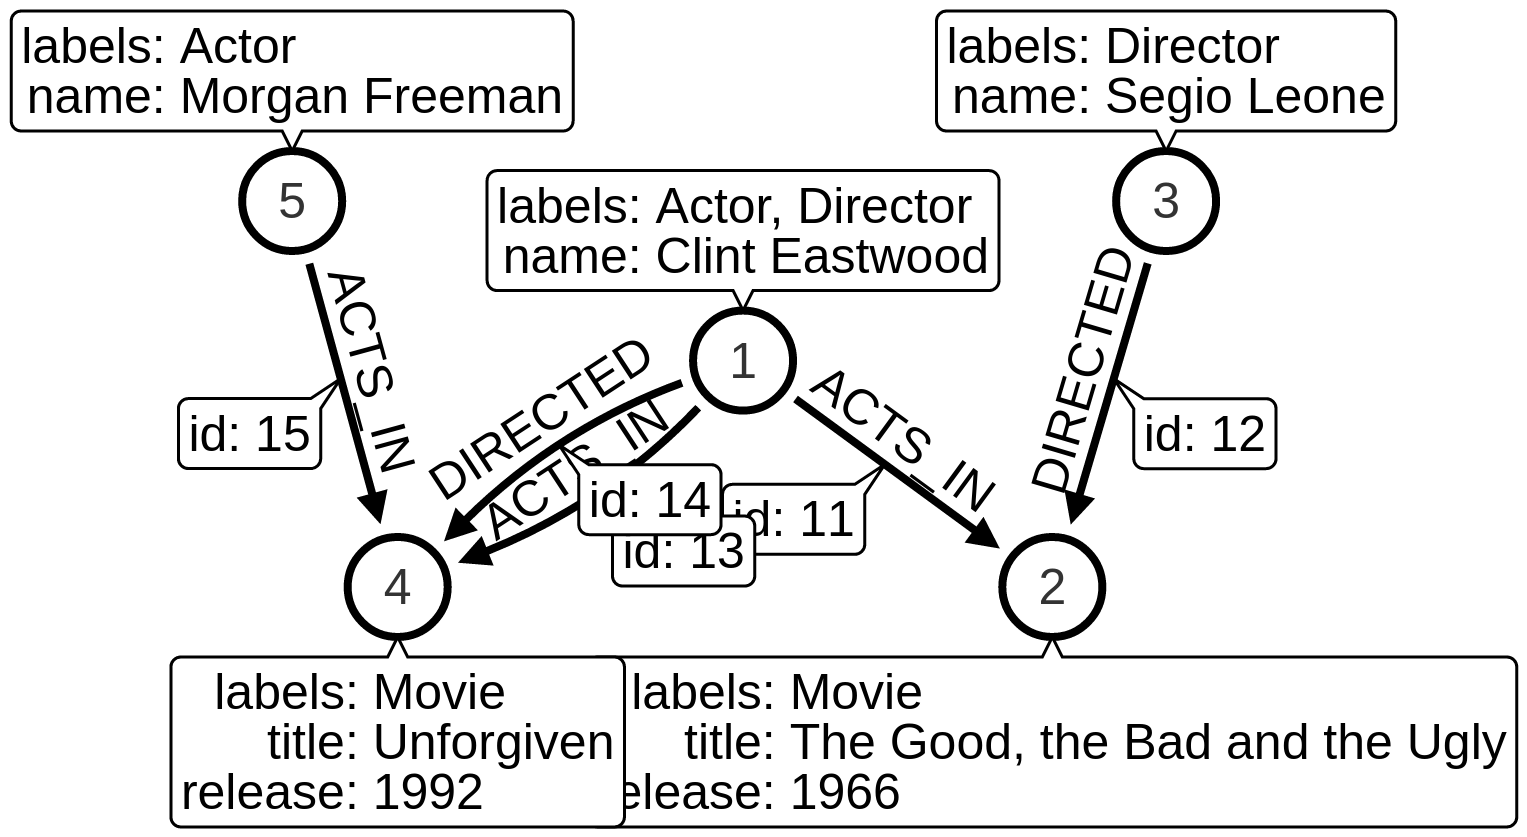
\includegraphics[width=6cm]{figures/movie-graph}
	\caption{Example movie graph.}
	\label{fig:running-example-property-graph}
\end{figure}

\paragraph{Running example.} \autoref{fig:running-example-property-graph} presents an example inspired by the Movie Database dataset\footnote{\url{https://neo4j.com/developer/movie-database/}}. The graph can be represented formally as:

\begin{minipage}{\textwidth}
	$V=\{1, 2, 3, 4, 5\}; E=\{11,12,13,14,15\};$
	
	$\verticestoedges(11) = \tuple{1, 2}; \verticestoedges(12) = \tuple{3, 2}; \ldots$

	$\vertexlabels = \{\atom{Actor}, \atom{Director}, \atom{Movie}\};$

	$\edgelabels = \{\atom{ACTS\_IN}, \atom{DIRECTED}\};$

	$\vertexlabelfunction(1) = \{\atom{Actor}, \atom{Director}\}; \vertexlabelfunction(2) = \{\atom{Movie}\}; \ldots;$

	$\edgelabelfunction(11) = \atom{ACTS\_IN}; \edgelabelfunction(12) = \atom{DIRECTED}; \ldots;$

	$\vertexproperties = \{\atom{name}, \atom{title}, \atom{release}\}; \edgeproperties = \{\};$

	$\propertyfunction{name}{1} = \atom{'Clint~Eastwood'}; \propertyfunction{name}{2} = \relnull; \ldots$

	$\propertyfunction{title}{1} = \relnull; \propertyfunction{title}{2} = \atom{'The~Good,~the~Bad~and~the~Ugly'}; \ldots$
	
	$\propertyfunction{release}{1} = \relnull; \propertyfunction{release}{2} = \atom{1966}; \ldots$
\end{minipage}

In the context of this paper, we define a \emph{relation} as a bag (\emph{multiset}) of tuples: a tuple can occur more than once in the relation~\cite{DBLP:books/daglib/0020812}.
Given a property graph $G$, relation $r$ is a \emph{graph relation} if the following holds:
$$\forall A \in \attr{r}: \dom{A} \subseteq V \union E \union D,$$
where $\attr{r}$ is the set of attributes of $r$, $\dom{A}$ is the domain of attribute $A$. The schema of $r$, $\schema{r}$ is a list containing the attribute names. For schema transformations, the \appendtext operator is denoted by $\append$, the \removetext operator is denoted by $\remove$.

\section{Operators of Relational Algebra}

For well-known relational algebra operators (\eg selection, projection, join) and common extensions (\eg aggregation, left outer join), we only give a brief summary. A more detailed discussion is available in database textbooks, \eg~\cite{DBLP:books/daglib/0020812, DBLP:books/daglib/0006733}.

We also adapted graph-specific operators from~\cite{DBLP:conf/edbt/HolschG16}\footnote{The \textsc{GetNodes} operator introduced in~\cite{DBLP:conf/edbt/HolschG16} and did not support labels. We extended it by allowing the specification of vertex labels and renamed it to \getverticestext to be consistent with the rest of the definitions. We also extended the \textsc{ExpandIn} and \textsc{ExpandOut} operators to allow it to return a set of edges, and introduced the \expandbothtext operator to allow navigation to both directions.} and propose new operators.

\subsection{Nullary Operators}
\label{sec:nullary-operators}

The \getverticestext nullary operator $\getvertices{v}{t_1 \land \ldots \land t_n}$ returns a graph relation of a single attribute $v$ that contains the ID of all vertices that have \emph{all} of labels $t_1, \ldots, t_n$.

\subsection{Unary Operators}
\label{sec:unary-operators}

The \projectiontext operator $\projectionop$ keeps a specific set of attributes in the relation: $ t = \projection{A_1, \ldots, A_n} \left(r\right).$ Note that the tuples are not deduplicated by default, \ie the results will have the same number of tuples as the input relation $r$. The projection operator can also rename the attributes, \eg $\projection{v1 \assign v2} \left(r\right)$ renames $\atom{v1}$ to $\atom{v2}$.

The \selectiontext operator $\selectionop$ filters the incoming relation according to some criteria. Formally,
$ t = \selection{\theta} \left(r\right), $
where predicate $\theta$ is a propositional formula. The operator selects all tuples in $r$ for which $\theta$ holds.

The \duplicateeliminationtext operator $\duplicateeliminationop$ eliminates duplicate tuples in a bag.

The \groupingtext operator $\groupingop$ groups tuples according to their value in one or more attributes and aggregates the remaining attributes. %Aggregated values (scalars and inline collections) makes \rga not closed under \groupingtext.

The \sorttext operator $\sortop$ transforms a bag relation of tuples to a list of tuples by ordering them. The ordering is defined by specified attributes of the tuples with an ordering direction (ascending $\asc$/descending $\desc$) for each attribute, \eg $\sort{\asc \atom{v1}, \desc \atom{v2}} (r)$.

The \toptext operator $\topp{l}{s}$ (adapted from~\cite{DBLP:conf/sigmod/LiCIS05}) takes a list as its input, skips the top $s$ tuples and returns the next $l$ tuples.\footnote{SQL implementations offer the \texttt{OFFSET} and the \texttt{LIMIT}/\texttt{TOP} keywords.}

The \expandbothtext operator $\expandboth{E}{l_1 \lor \ldots \lor l_k \ast min \ldots max}{v}{w}{t_1 \land \ldots \land t_n}{min}{max}(r)$ adds (1)~a new attribute $w$ to $r$ containing the IDs of vertices having \emph{all} labels $t_1, \ldots, t_n$ that can be reached from vertices of attribute $v$ by traversing edges having \emph{any} labels $l_1, \ldots, l_n$, and (2)~a new attribute $E$ for the edges of the path from $v$ to $w$. The operator may use at least $\atom{min}$ and at most $\atom{max}$ hops, both defaulting to $1$ if omitted. % With the default setting, \ie $\atom{min}=\atom{max}=1$, a single edge variable $e$ can be used instead of edge list $E$.
The \expandintext operator~$\expandinop$ and \expandouttext operator~$\expandoutop$ only consider directed paths from $w$ to $v$ and from $v$ to $w$, respectively.

The \unwindtext operator $\unwind{xs}{x}$ unfolds a list $\atom{xs}$ to a variable $\atom{x}$ by introducing additional rows, each containing a single element of the list.

The \alldifferenttext operator $\alldifferent{E_1, E_2, E_3, \ldots}{(r)}$ filters $r$ to keep tuples where the variables in $\bigcup_{i} E_{i}$ are pairwise different.\footnote{Should e.g. $E_2$ be a set of the single variable $e_2$, the variable name can be used as a shorthand instead, so $\alldifferent{E_1, e_2, E_3, \ldots}{(r)} ~ \equiv ~ \alldifferent{E_1, \{e_2\}, E_3, \ldots}{(r)}$}
It can be expressed as a \selectiontext:
$$\alldifferent{E_1, E_2, E_3, \ldots}{(r)} = \selection{ \bigwedge\limits_{e_1, e_2 \,\in\, \bigcup\limits_{i} {E_i} ~ \wedge ~ { e_1 \,\neq\, e_2 } } { r.e_1 \,\neq\, r.e_2 } }{(r)}$$

We use the \alldifferenttext operator to guarantee the uniqueness of edges (see the remark on \emph{uniqueness of edges} in \autoref{sec:opencypher}).

\subsection{Binary Operators}
\label{sec:binary-operators}

The $\unionop$ operator produces the set union of two relations, while the $\bagunionop$ operator produces the \emph{bag union} of two operators, \eg $\{\tuple{1, 2}, \tuple{1, 2}, \tuple{3, 4}\} \bagunionop \{\tuple{1, 2}\} = \{\tuple{1, 2}, \tuple{1, 2}, \tuple{1, 2}, \tuple{3, 4}\}$. For both the \uniontext and \baguniontext operators, the schema of the operands must have the same number of attributes. Some authors also require that they share a common schema, \ie have the same set of attributes~\cite{DBLP:books/daglib/0020812}.

The $\cartesianproductop$ operator produces the \cartesianproducttext:

$$ t = r \cartesianproductop s.$$

The result of the \jointext operator $\joinop$ is determined by creating the Cartesian product of the relations, then filtering those tuples which are equal on the attributes that share a common name. The combined tuples are projected: from the attributes present in both of the two input relations, we only keep the ones in $r$ and drop the ones in $s$. Thus, the join operator is defined as
$$r \join s = \pi_{R \union S} \left(\selection{r.A_1 = s.A_1\,\land\,\ldots\,\land\,r.A_n = s.A_n)} \left(r \times s\right) \right),$$
where $ \{ A_1, \ldots, A_n \} $ is the set of attributes that occur both in $R$ and $S$, \ie $ R \intersection S = \{ A_1, \ldots, A_n \} $. Note that if the set of common attributes is empty, the \jointext operator is equivalent to the Cartesian product of the relations.
The join operator is both commutative and associative: $r \join s = s \join r$ and $(r \join s) \join t = r \join (s \join t)$, respectively.

The \antijointext operator $\antijoinop$ (also known as \emph{left anti semijoin}) collects the tuples from the left relation $r$ which have no matching pair in the right relation $s$:
$$ t = r \antijoin s = r \setminus \pi_{R} \left(r \join s\right), $$
where $\pi_{R}$ denotes a projection operator, which only keeps the attributes of the schema over relation $r$. The antijoin operator is not commutative and not associative.

The \leftouterjointext $\myleftouterjoin$ pads tuples from the left relation that did not match any from the right relation with $\relnull$ values and adds them to the result of the \jointext~\cite{DBLP:books/daglib/0015084}:
$$ t = r \myleftouterjoin s = (r \join s) \union (r \antijoin s) \cartesianproductop \{\relnull, \ldots, \relnull\}, $$

where the constant relation $\{\relnull, \ldots, \relnull\}$ is on the schema $S \setminus R$.

\subsection{Property Access}

Assuming that $x$ is an attribute of a graph relation, we use the notation $x.a$ in (1)~attribute lists for projections and (2)~selection conditions to express the access to the corresponding value of property $a$ in the property graph~\cite{DBLP:conf/edbt/HolschG16}.

\subsection{Summary of Operators}

\autoref{table:collections} provides an overview of the operators of \rga.

\newcommand{\propheader}{\multirow{2}{*}{\bf prop.}}
\newcommand{\rgaheader}{\multirow{2}{*}{\breakable{\bf RGA}}}

\setlength\tabcolsep{3.6pt}
\begin{table}[htb]
	\centering
	\begin{tabular}{||c||c|c|c||c|c|c||c||c||}
		\hline
		\multirow{2}{*}{\bf ops} &             \multirow{2}{*}{\bf operator}             &         \multirow{2}{*}{\bf name}         & \propheader & \multicolumn{3}{c||}{\bf output for} &             \multirow{2}{*}{\bf schema}              \\ \cline{5-7}
		&                                                       &                                           &             & \bf set & \bf bag &     \bf list     &  \\ \hline\hline
		\multirow{1}{*}{\bf 0}   &                  $\getvertices{v}{}$                  &             \getverticestext              &     set     &   set   &   set   &       set        &                  $\tuple{\atom{v}}$                  \\ \hline\hline %\cline{2-8}
%		&              $\getedges{v}{}{w}{}{e}{}$               &               \getedgestext               &     $-$     &   $-$   &   $-$   &       $-$        &               $\tuple{\atom{v, e, w}}$               \\ \hline\hline
		\multirow{8}{*}{\bf 1}   &         $\projection{v_1, v_2, \ldots} (r)$         &              \projectiontext              &      i      &   bag   &   bag   &       list       &         $\tuple{\atom{v_1, v_2, \ldots}}$          \\ \cline{2-8}
		&              $\selection{condition} (r)$              &              \selectiontext               &      i      &   set   &   bag   &       list       &                     $\schema{r}$                     \\ \cline{2-8}
		&            $\expandboth{v}{w}{}{e}{}{min}{max} (r)$             &              \expandbothtext              &     $-$     &   set   &   bag   &       list       &       $\schema{r} \append \tuple{\atom{e, w}}$       \\ \cline{2-8}
		&            $\alldifferent{variables} (r)$             &             \alldifferenttext             &      i      &   set   &   bag   &       list       &                     $\schema{r}$                     \\ \cline{2-8}
		&             $\duplicateeliminationop (r)$             &         \duplicateeliminationtext         &      i      &   set   &   set   &       list       &                     $\schema{r}$                     \\ \cline{2-8}
		&                     $\sort{\desc \atom{v_1}, \asc \atom{v_2}, \ldots} (r)$                     &                 \sorttext                 &      i      &  list   &  list   &       list       &                     $\schema{r}$                     \\ \cline{2-8}
		&          $\grouping{v_1, v_2, \ldots} (r)$          &               \groupingtext               &      i      &   set   &   set   &       set        &         $\tuple{\atom{v_1, v_2, \ldots}}$          \\ \cline{2-8}
		&                     $\topop (r)$                      &                 \toptext                  &     $-$     &  list   &  list   &       list       &                     $\schema{r}$                     \\ \hline\hline
		\multirow{5}{*}{\bf 2}   & $r \unionop s$, $r \minusop s$ & \uniontext, \minustext &     $-$     &   set   &   set   &       set        &                     $\schema{r}$                     \\ \cline{2-8}
		&                    $r \bagunion s$                    &               \baguniontext               &    c, a     &   bag   &   bag   &       bag        &                     $\schema{r}$                     \\ \cline{2-8}
		&               $r \cartesianproductop s$               &           \cartesianproducttext           &    c, a     &   set   &   bag   &       bag        &           $\schema{r} \append \schema{s}$            \\ \cline{2-8}
		&                    $r \joinop s$                      &                 \jointext                 &    c, a     &   set   &   bag   &       bag        & $\schema{r} \append (\schema{s} \minus \schema{r}) $ \\ \cline{2-8}
		&                $r \myleftouterjoin s$                 &            \leftouterjointext             &     $-$     &   set   &   bag   &       bag        & $\schema{r} \append (\schema{s} \minus \schema{r}) $ \\ \cline{2-8}
		&                   $r \antijoinop s$                   &               \antijointext               &    c, a     &   set   &   bag   &       bag        &                     $\schema{r}$                     \\ \cline{1-8}
	\end{tabular}
	\caption{Properties of relational graph algebra operators. A unary operator $\alpha$ is idempotent~(i), iff $\alpha(x) = \alpha(\alpha(x))$ for all inputs. A binary operator $\beta$ is commutative~(c), iff $x~\beta~y = y~\beta~x$ and associative~(a), iff $(x~\beta~y)~\beta~z = x~\beta~(y~\beta~z)$.}
	\label{table:collections}
\end{table}
